\documentclass[12pt, letterpaper]{article} 
\usepackage{graphicx} 
\usepackage{hyperref} 
\usepackage[utf8]{inputenc} 
\usepackage{float} 
\usepackage{geometry} 
\usepackage{enumitem, array} 
\usepackage{longtable} 
\usepackage{lscape} 
\usepackage[export]{adjustbox} 
\geometry{letterpaper, left=10mm, right=10mm, bottom=20mm, top=20mm} 
\graphicspath{{../img/simulation/}} 
\renewcommand{\rule}{Rule 30} 
\renewcommand{\r}{30} 
\title{Rule 30 report} 
\author{Fi Simulator} 
\begin{document} 
\begin{titlepage} 
\maketitle 
\tableofcontents 
\end{titlepage} 
\clearpage 
\begin{figure}[H]
	\centering
	\includegraphics[height=200mm, width=200mm, keepaspectratio]{simAnalysis.png} 
	\caption{Rule 30 evolution} 
\end{figure}
\begin{table}[H]
	\centering
	\begin{tabular}{|c|c|c|c| }
		\hline Seed-Density & Fill & Length & Steps \\ 
			\hline 50 &  & 512 & 256 \\ 
			\hline 
	\end{tabular} 
	\caption{Simulation data} 
\end{table} 
\begin{section}{Phenotypic Analysis} 
	\begin{subsection}{Density} 
		\begin{figure}[H] 
		\centering 
				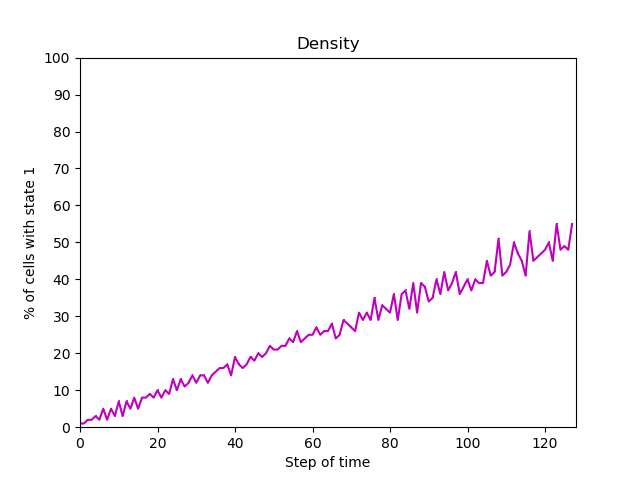
\includegraphics[max width=200mm, max height=200mm, keepaspectratio]{SimDensity.png} 
			\caption{Density plot} 
		\end{figure} 
	\end{subsection} 
Density plot shows the percentage of cells with state 1 along every step of time in the simulation	\begin{subsection}{Entropy} 
		\begin{figure}[H] 
		\centering 
			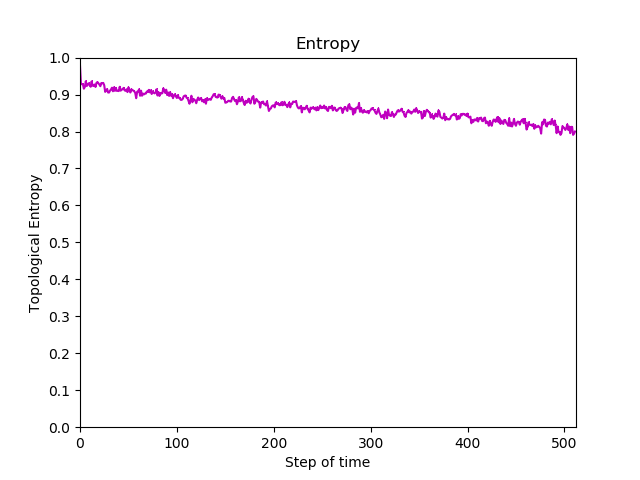
\includegraphics[max width=200mm, max height=200mm, keepaspectratio]{SimEntropy.png} 
		\caption{Entropy plot} 
		\end{figure} 
	\end{subsection}
Entropy plot shows the information in the system along every step of time in the simulation, the more information higher the entropy and the system can be considered more chaotic	\begin{subsection}{Lyapunov exponents} 
		\begin{figure}[H] 
		\centering 
			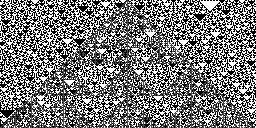
\includegraphics[max width=200mm, max height=200mm, keepaspectratio]{SimDefects.png} 
		\caption{Damage spreading} 
		\end{figure} 
	\end{subsection} 
	\begin{table}[H] 
	\centering 
		\begin{tabular}{cc} 
			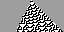
\includegraphics[width=70mm, max height=70mm, keepaspectratio]{SimOriginal.png} & 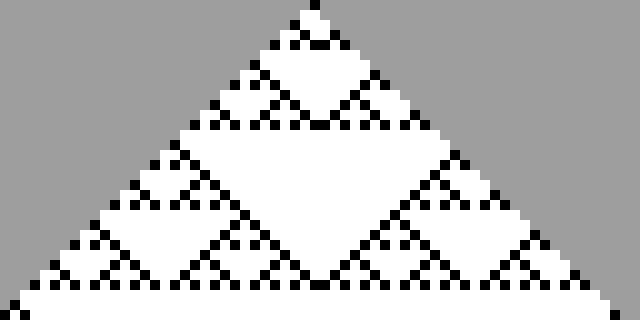
\includegraphics[width=70mm, max height=70mm, keepaspectratio]{SimAlter.png} \ 
		\end{tabular} 
		\caption{Original simulation and Altered simulation comparison} 
	\end{table} 
	\begin{figure}[H] 
		\centering 
			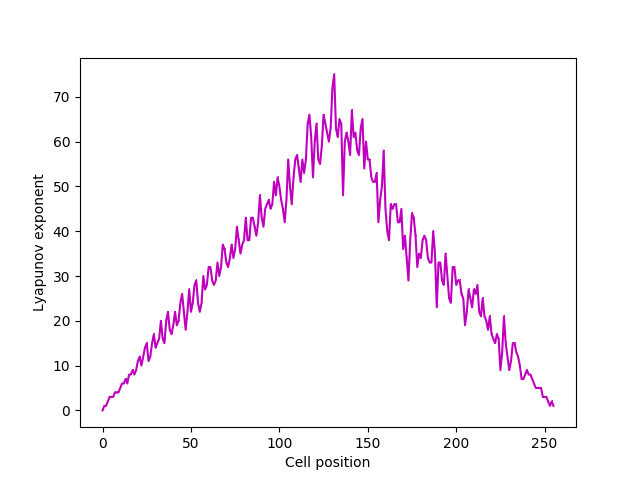
\includegraphics[max width=200mm, max height=200mm, keepaspectratio]{SimLyapunovExp.png} 
		\caption{Lyapunov profile} 
		\end{figure} 
The Lyapunov analysis shows the time-averaged expansions rates in each possible direction of a single defect introduced in the initial configuration.    \end{section} 
    \clearpage 
\end{document}